\documentclass[t,usenames,dvipsnames]{beamer}
\usetheme{Copenhagen}
\setbeamertemplate{headline}{} % remove toc from headers
\beamertemplatenavigationsymbolsempty

\usepackage{amsmath, xcolor, tikz, pgfplots, bm}

\pgfplotsset{compat = 1.16}
\usetikzlibrary{arrows.meta, calc, decorations.pathreplacing}
\pgfplotsset{every axis/.append style = {axis lines = middle}}
\pgfplotsset{every tick label/.append style={font=\scriptsize}}
\everymath{\displaystyle}

\title{Dividing Polynomials}
\author{}
\date{}

\AtBeginSection[]
{
  \begin{frame}
    \frametitle{Objectives}
    \tableofcontents[currentsection]
  \end{frame}
}

\begin{document}

\begin{frame}
    \maketitle
\end{frame}

\section{Divide polynomials without a remainder}

\begin{frame}{Division Basics}
In the expression $a \div b = c$, $a$ is the \alert{dividend}, $b$ is the \alert{divisor}, and $c$ is the \alert{quotient}.   \newline\\

When dividing polynomials, it will help to write your terms in standard form (descending powers). You may also need to fill in any missing terms using 0 as a coefficient. \newline\\

Before we get to division, let's review an organizational technique for multiplying polynomials.
\end{frame}

\begin{frame}{Multiplication Example}
To find the product of $(x-2)(x^2+6x+7)$, we can use the following method:   
\begin{center}
    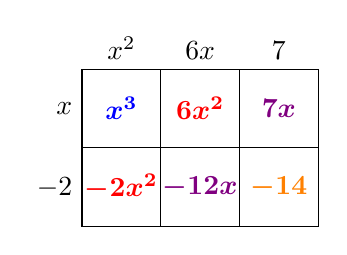
\begin{tikzpicture}
    \draw (0,0) grid (3,2);
    \node at (0,1.5) [left] {$x$};
    \node at (0,0.5) [left] {$-2$};
    \node at (0.5,2) [above] {$x^2$};
    \node at (1.5,2) [above] {$6x$};
    \node at (2.5,2) [above] {7};
    \onslide<2->{\node at (0.5,1.5) {\color{blue}$\bm{x^3}$};}
    \onslide<4->{\node at (1.5,1.5) {\color{red}$\bm{6x^2}$};}
    \onslide<3->{\node at (0.5,0.5) {\color{red}$\bm{-2x^2}$};}
    \onslide<5->{\node at (1.5,0.5) {\color{violet}$\bm{-12x}$};}
    \onslide<6->{\node at (2.5,1.5) {\color{violet}$\bm{7x}$};}
    \onslide<7->{\node at (2.5,0.5) {\color{orange}$\bm{-14}$};}
    \end{tikzpicture}
\end{center}
\onslide<8->{
When we combine all of terms inside the box, we get the product, $x^3 + 4x^2 - 5x - 14$.}
\end{frame}

\begin{frame}{Division}
We can reverse the process using division to find the quotient
\[
(x^3 + 4x^2 - 5x - 14) \div (x - 2)
\]
\begin{center}
    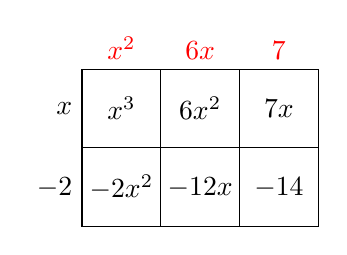
\begin{tikzpicture}
    \draw (0,0) grid (3,2);
    \node at (0,1.5) [left] {$x$};
    \node at (0,0.5) [left] {$-2$};
    \node at (0.5,1.5) {$x^3$};
    \onslide<2->{\node at (0.5,2) [above] {\color{red}$x^2$};}
    \onslide<3->{\node at (0.5,0.5) {$-2x^2$};}
    \onslide<4->{\node at (1.5,1.5) {$6x^2$};}
    \onslide<5->{\node at (1.5,2) [above] {\color{red}$6x$};}
    \onslide<6->{\node at (1.5,0.5) {$-12x$};}
    \onslide<8->{\node at (2.5,2) [above] {\color{red}$7$};}
    \onslide<7->{\node at (2.5,1.5) {$7x$};}
    \onslide<9->{\node at (2.5,0.5) {$-14$};}
\end{tikzpicture}
\end{center}
\onslide<10->{\[x^2 + 6x + 7\]}
\end{frame}

\begin{frame}{Example 1}
Divide $(x^3+8) \div (x+2)$
\onslide<2->{\[(x^3 + 0x^2 + 0x + 8) \div (x+2)\]}
\begin{center}
\onslide<3->{
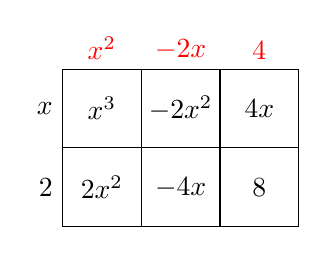
\begin{tikzpicture}
\draw (0,0) grid (3,2);
\node at (0,1.5) [left] {$x$};
\node at (0,0.5) [left] {2};
\onslide<4->{\node at (0.5,1.5) {$x^3$};}
\onslide<5->{\node at (0.5,2) [above] {\color{red}$x^2$};}
\onslide<6->{\node at (0.5,0.5) {$2x^2$};}
\onslide<7->{\node at (1.5,1.5) {$-2x^2$};}
\onslide<8->{\node at (1.5,2) [above] {\color{red}$-2x$};}
\onslide<9->{\node at (1.5,0.5) {$-4x$};}
\onslide<10->{\node at (2.5,1.5) {$4x$};}
\onslide<11->{\node at (2.5,2) [above] {\color{red}4};}
\onslide<12->{\node at (2.5,0.5) {8};}
\end{tikzpicture}} \vspace{8pt}
\end{center}
\onslide<13->{\[\color{red}{x^2 - 2x + 4}\]}
\end{frame}


\section{Divide polynomials with a remainder}

\begin{frame}{Dividing Polynomials With a Remainder}
In the previous examples, everything ``balanced out" from within the grid. \newline\\

In other words, after combining like terms, all terms in the dividend were accounted for.    \newline\\  \pause

In the next group of examples, we will need to figure out what to add to our quotient to ``balance out the problem."  \newline\\  

We will write our answers in the form 
\[
\text{quotient} + \frac{\text{remainder}}{\text{divisor}}
\]
\end{frame}

\begin{frame}{Example 2}
Divide each.    \newline\\
(a) \quad $(5x^3 - 2x^2 + 1) \div (x-3)$
\onslide<2->{\[(5x^3 - 2x^2 + 0x + 1) \div (x-3) \]}
\onslide<3->{
\begin{center}
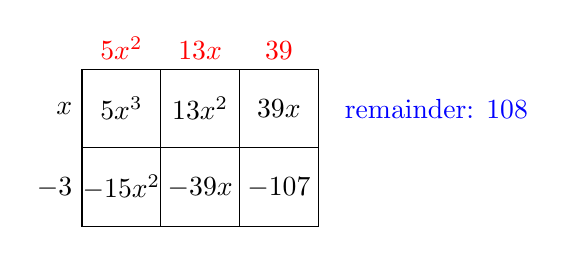
\begin{tikzpicture}
\draw (0,0) grid (3,2);
\node at (0,1.5) [left] {$x$};
\node at (0,0.5) [left] {$-3$};
\onslide<4->{\node at (0.5,1.5) {$5x^3$};}
\onslide<5->{\node at (0.5,2) [above] {\color{red}$5x^2$};}
\onslide<6->{\node at (0.5,0.5) {$-15x^2$};}
\onslide<7->{\node at (1.5,1.5) {$13x^2$};}
\onslide<8->{\node at (1.5,2) [above] {$\color{red}13x$};}
\onslide<9->{\node at (1.5,0.5) {$-39x$};}
\onslide<10->{\node at (2.5,1.5) {$39x$};}
\onslide<11->{\node at (2.5,2) [above] {$\color{red}39$};}
\onslide<12->{\node at (2.5,0.5) {$-107$};}
\onslide<13->{\node at (4.5,1.5) {$\color{blue}\text{remainder: }108$};}
\end{tikzpicture}
\end{center}}
\end{frame}


\begin{frame}{Example 2}
(a) \quad $(5x^3 - 2x^2 + 1) \div (x-3)$

\[ 5x^2 + 13x + 39 \text{ remainder: } 108  \]  \vspace{12pt}   \pause

\[ 5x^2 + 13x + 39 + \frac{108}{x-3} \]
\end{frame}

\begin{frame}{Example 2}
(b) \quad $(4-8x-12x^2) \div (2x-3)$
\onslide<2->{\[(-12x^2 - 8x + 4) \div (2x-3)\]}
\onslide<3->{
\begin{center}
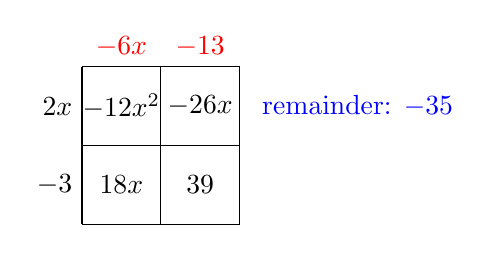
\begin{tikzpicture}
\draw (0,0) grid (2,2);
\node at (0,1.5) [left] {$2x$};
\node at (0,0.5) [left] {$-3$};
\onslide<4->{\node at (0.5,1.5) {$-12x^2$};}
\onslide<5->{\node at (0.5,2) [above] {\color{red}$-6x$};}
\onslide<6->{\node at (0.5,0.5) {$18x$};}
\onslide<7->{\node at (1.5,1.5) {$-26x$};}
\onslide<8->{\node at (1.5,2) [above] {$\color{red}-13$};}
\onslide<9->{\node at (1.5,0.5) {$39$};}
\onslide<10->{\node at (3.5,1.5) {\color{blue}\text{remainder: }$-35$};}
\end{tikzpicture}
\end{center}}
\end{frame}

\begin{frame}{Example 2}
(b) \quad $(4-8x-12x^2) \div (2x-3)$
\[-6x - 13 \text{remainder } -35 \] \pause
\[ -6x - 13 - \frac{35}{2x-3}\]
\end{frame}

\begin{frame}{Example 2}
(c) \quad   $(3x^3 + 4x^2 + x + 7) \div (x^2 + 1)$  
\onslide<2->{\[(3x^3 + 4x^2 + x + 7) \div (x^2 + 0x + 1)\]}
\onslide<3->{
\begin{center}
    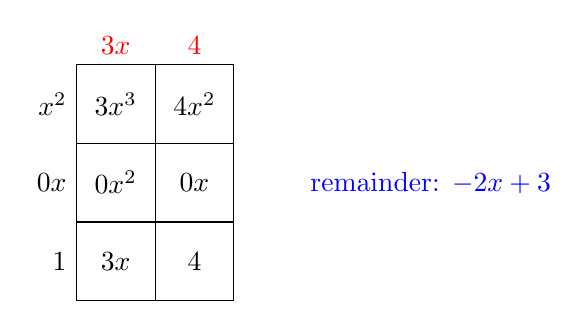
\begin{tikzpicture}
    \draw (0,0) grid (2,3);
    \node at (0,2.5) [left] {$x^2$};
    \node at (0,1.5) [left] {$0x$};
    \node at (0,0.5) [left] {$1$};
    \node at (0.5,2.5) {$3x^3$};
    \onslide<7->{\node at (1.5,2.5) {$4x^2$};}
    \onslide<5->{\node at (0.5,1.5) {$0x^2$};}
    \onslide<9->{\node at (1.5,1.5) {$0x$};}
    \onslide<6->{\node at (0.5,0.5) {$3x$};}
    \onslide<10->{\node at (1.5,0.5) {4};}
    \onslide<4->{\node at (0.5,3) [above] {\color{red}$3x$};}
    \onslide<8->{\node at (1.5,3) [above] {\color{red}$4$};}
    \onslide<11->{\node at (4.5,1.5) {\color{blue}\text{remainder: }$-2x+3$};}
\end{tikzpicture}
\end{center}}
\end{frame}

\begin{frame}{Example 2}
(c) \quad   $(3x^3 + 4x^2 + x + 7) \div (x^2 + 1)$ 
\[ 3x + 4 \text{remainder } -2x+3 \]
\onslide<2->{\[3x + 4 + \frac{-2x+3}{x^2+1}\]}
\end{frame}

\section{Find the remainder of polynomial division using the Remainder Theorem}
\section{Determine if a divisor is a factor of a dividend using the Factor Theorem}

\end{document}


% \iffalse

% Dividing is nothing more than the inverse operation of multiplication. In other words, it can get you back to where you started from when multiplying.  \newline\\

% When dividing polynomials, it will help to write your terms in standard form (descending powers).  \newline\\

% Before we get to division, let's review an organizational technique for multiplying polynomials.    \newline\\

% To find the product of $(x-2)(x^2+6x+7)$, we can use the following method:   
% \begin{center}
%     \begin{tikzpicture}
%     \draw (0,0) grid (3,2);
%     \node at (0,1.5) [left] {$x$};
%     \node at (0,0.5) [left] {$-2$};
%     \node at (0.5,2) [above] {$x^2$};
%     \node at (1.5,2) [above] {$6x$};
%     \node at (2.5,2) [above] {7};
%     \node at (0.5,1.5) {\color{blue}$\bm{x^3}$};
%     \node at (1.5,1.5) {\color{red}$\bm{6x^2}$};
%     \node at (0.5,0.5) {\color{red}$\bm{-2x^2}$};
%     \node at (1.5,0.5) {\color{violet}$\bm{-12x}$};
%     \node at (2.5,1.5) {\color{violet}$\bm{7x}$};
%     \node at (2.5,0.5) {\color{orange}$\bm{-14}$};
%     \end{tikzpicture}
% \end{center}

% Notice the like terms (color-coded) along the diagonals inside the box. The upper left of the box, $\color{blue}x^3$, and the bottom right of the box, $\color{orange}-14$, have no like terms inside the boxes.  \newline\\

% When we combine all of terms inside the box, we get the quotient, $x^3 + 4x^2 - 5x - 14$.    \newline\\

% We can reverse the process using division to find the quotient
% \[
% (x^3 + 4x^2 - 5x - 14) \div (x - 2)
% \]

% First, let's look at the upper-left portion of the box:
% \begin{center}
% \begin{tikzpicture}
%     \draw (0,0) grid (1,2);
%     \node at (0,1.5) [left] {$x$};
%     \node at (0,0.5) [left] {$-2$};
%     \node at (0.5,1.5) {\color{blue}$\bm{x^3}$};
% \end{tikzpicture}
% \end{center}

% To find the value that will go above the first column, divide $x^3$ by $x$ to get $x^2$.

% \begin{center}
% \begin{tikzpicture}
%     \draw (0,0) grid (1,2);
%     \node at (0,1.5) [left] {$x$};
%     \node at (0,0.5) [left] {$-2$};
%     \node at (0.5,1.5) {$x^3$};
%     \node at (0.5,2) [above] {\color{red}$x^2$};
% \end{tikzpicture}
% \end{center}

% Now, multiply the $-2$ and the $x^2$ to fill in the bottom cell:
% \begin{center}
%     \begin{tikzpicture}
%     \draw (0,0) grid (1,2);
%     \node at (0,1.5) [left] {$x$};
%     \node at (0,0.5) [left] {$-2$};
%     \node at (0.5,1.5) {$x^3$};
%     \node at (0.5,2) [above] {\color{red}$x^2$}; table
%     \node at (0.5,0.5) {$-2x^2$};
% \end{tikzpicture}
% \end{center}

% Next, let's go to the second column:
% \begin{center}
%     \begin{tikzpicture}
%     \draw [fill=yellow!60] (1,1) rectangle (2,2);
%     \draw (0,0) grid (2,2);
%     \node at (0,1.5) [left] {$x$};
%     \node at (0,0.5) [left] {$-2$};
%     \node at (0.5,1.5) {$x^3$};
%     \node at (0.5,2) [above] {\color{red}$x^2$};
%     \node at (0.5,0.5) {$-2x^2$};
% \end{tikzpicture}
% \end{center}

% The $-2x^2$ and the highlighted cell must combine to make the $4x^2$ term in the dividend. Thus, the highlighted cell's value must be $6x^2$, since $-2x^2 + 6x^2 = 4x^2$.
% \begin{center}
%     \begin{tikzpicture}
%     \draw [fill=yellow!60] (1,1) rectangle (2,2);
%     \draw (0,0) grid (2,2);
%     \node at (0,1.5) [left] {$x$};
%     \node at (0,0.5) [left] {$-2$};
%     \node at (0.5,1.5) {$x^3$};
%     \node at (0.5,2) [above] {\color{red}$x^2$};
%     \node at (0.5,0.5) {$-2x^2$};
%     \node at (1.5,1.5) {$\bm{6x^2}$};
% \end{tikzpicture}
% \end{center}

% Now, to get the value that will go above the 2nd column, divide the $6x^2$ by $x$ to get $6x$:
% \begin{center}
%     \begin{tikzpicture}
%     \draw (0,0) grid (2,2);
%     \node at (0,1.5) [left] {$x$};
%     \node at (0,0.5) [left] {$-2$};
%     \node at (0.5,1.5) {$x^3$};
%     \node at (0.5,2) [above] {\color{red}$x^2$};
%     \node at (0.5,0.5) {$-2x^2$};
%     \node at (1.5,1.5) {\color{blue}$\bm{6x^2}$};
%     \node at (1.5,2) [above] {\color{red}$6x$};
% \end{tikzpicture}
% \end{center}

% The bottom right cell will be $6x(-2) = -12x$:
% \begin{center}
%     \begin{tikzpicture}
%     \draw (0,0) grid (2,2);
%     \node at (0,1.5) [left] {$x$};
%     \node at (0,0.5) [left] {$-2$};
%     \node at (0.5,1.5) {$x^3$};
%     \node at (0.5,2) [above] {\color{red}$x^2$};
%     \node at (0.5,0.5) {$-2x^2$};
%     \node at (1.5,1.5) {$6x^2$};
%     \node at (1.5,2) [above] {\color{red}$6x$};
%     \node at (1.5,0.5) {$-12x$};
% \end{tikzpicture}
% \end{center}

% Lastly, we go to the next column:
% \begin{center}
%     \begin{tikzpicture}
%     \draw [fill=yellow!60] (2,1) rectangle (3,2);
%     \draw (0,0) grid (3,2);
%     \node at (0,1.5) [left] {$x$};
%     \node at (0,0.5) [left] {$-2$};
%     \node at (0.5,1.5) {$x^3$};
%     \node at (0.5,2) [above] {\color{red}$x^2$};
%     \node at (0.5,0.5) {$-2x^2$};
%     \node at (1.5,1.5) {$6x^2$};
%     \node at (1.5,2) [above] {\color{red}$6x$};
%     \node at (1.5,0.5) {$-12x$};
% \end{tikzpicture}
% \end{center}

% The highlighted cell will combine with the $-12x$ to produce $-5x$. That means the highlighted cell's value must be $7x$ since $7x-12x = -5x$.
% \begin{center}
%     \begin{tikzpicture}
%     \draw [fill=yellow!60] (2,1) rectangle (3,2);
%     \draw (0,0) grid (3,2);
%     \node at (0,1.5) [left] {$x$};
%     \node at (0,0.5) [left] {$-2$};
%     \node at (0.5,1.5) {$x^3$};
%     \node at (0.5,2) [above] {\color{red}$x^2$};
%     \node at (0.5,0.5) {$-2x^2$};
%     \node at (1.5,1.5) {$6x^2$};
%     \node at (1.5,2) [above] {\color{red}$6x$};
%     \node at (1.5,0.5) {$-12x$};
%     \node at (2.5,1.5) {$\bm{7x}$};
% \end{tikzpicture}
% \end{center}

% To get the value that goes above the 3rd column, divide $7x$ by $x$ to get 7.
% \begin{center}
%     \begin{tikzpicture}
%     \draw (0,0) grid (3,2);
%     \node at (0,1.5) [left] {$x$};
%     \node at (0,0.5) [left] {$-2$};
%     \node at (0.5,1.5) {$x^3$};
%     \node at (0.5,2) [above] {\color{red}$x^2$};
%     \node at (0.5,0.5) {$-2x^2$};
%     \node at (1.5,1.5) {$6x^2$};
%     \node at (1.5,2) [above] {\color{red}$6x$};
%     \node at (1.5,0.5) {$-12x$};
%     \node at (2.5,2) [above] {\color{red}$7$};
%     \node at (2.5,1.5) {\color{blue}$\bm{7x}$};
% \end{tikzpicture}
% \end{center}

% Finally, multiply 7 by $-2$ to get $-14$ in the bottom right cell:
% \begin{center}
%     \begin{tikzpicture}
%     \draw (0,0) grid (3,2);
%     \node at (0,1.5) [left] {$x$};
%     \node at (0,0.5) [left] {$-2$};
%     \node at (0.5,1.5) {$x^3$};
%     \node at (0.5,2) [above] {\color{red}$x^2$};
%     \node at (0.5,0.5) {$-2x^2$};
%     \node at (1.5,1.5) {$6x^2$};
%     \node at (1.5,2) [above] {\color{red}$6x$};
%     \node at (1.5,0.5) {$-12x$};
%     \node at (2.5,2) [above] {\color{red}$7$};
%     \node at (2.5,1.5) {$7x$};
%     \node at (2.5,0.5) {$-14$};
% \end{tikzpicture}
% \end{center}

% Thus, the quotient is $\boxed{x^2 + 6x + 7}$.   \newline\\

% To check our answer, if we add all values inside the boxes, we get $x^3 + 4x^2 - 5x - 14$. Since that is also the dividend, our answer is correct \Smiley. \newline\\

% \textbf{Example 1.} Divide each of the following.   \newline\\

% (a) \quad   $(x^2 + 10x + 21) \div (x+3)$.  \newline\\

% Start by dividing $x^2$ by $x$ to get $x$. Then multiply $x$ by 3 to fill in the bottom cell:
% \begin{center}
%     \begin{tikzpicture}
%     \draw (0,0) grid (1,2);
%     \node at (0,1.5) [left] {$x$};
%     \node at (0,0.5) [left] {$3$};
%     \node at (0.5,1.5) {\color{blue}$\bm{x^2}$};
%     \node at (0.5,2) [above] {\color{red}$x$};
%     \node at (0.5,0.5) {$3x$};
% \end{tikzpicture}
% \end{center}

% The highlighted cell below must combine with $3x$ to produce $10x$, so it must be $7x$:
% \begin{center}
%     \begin{tikzpicture}
%     \draw [fill=yellow!60] (1,1) rectangle (2,2);
%     \draw (0,0) grid (2,2);
%     \node at (0,1.5) [left] {$x$};
%     \node at (0,0.5) [left] {$3$};
%     \node at (0.5,1.5) {$x^2$};
%     \node at (0.5,2) [above] {\color{red}$x$};
%     \node at (0.5,0.5) {$3x$};
%     \node at (1.5,1.5) {$\bm{7x}$};
% \end{tikzpicture}
% \end{center}

% Dividing $7x$ by $x$ yields a value of 7 above the 2nd column:
% \begin{center}
%     \begin{tikzpicture}
%     \draw (0,0) grid (2,2);
%     \node at (0,1.5) [left] {$x$};
%     \node at (0,0.5) [left] {$3$};
%     \node at (0.5,1.5) {$x^2$};
%     \node at (0.5,2) [above] {\color{red}$x$};
%     \node at (0.5,0.5) {$3x$};
%     \node at (1.5,1.5) {\color{blue}$\bm{7x}$};
%     \node at (1.5,2) [above] {\color{red}$7$};
% \end{tikzpicture}
% \end{center}

% The bottom left cell's value will be 21 ($7 \times 3$)
% \begin{center}
%     \begin{tikzpicture}
%     \draw (0,0) grid (2,2);
%     \node at (0,1.5) [left] {$x$};
%     \node at (0,0.5) [left] {$3$};
%     \node at (0.5,1.5) {$x^2$};
%     \node at (0.5,2) [above] {\color{red}$x$};
%     \node at (0.5,0.5) {$3x$};
%     \node at (1.5,1.5) {$7x$};
%     \node at (1.5,2) [above] {\color{red}$7$};
%     \node at (1.5,0.5) {$21$};
% \end{tikzpicture}
% \end{center}

% All of the terms inside the boxes combine to make $x^2 + 10x + 21$, so we are finished. The quotient is $\boxed{x + 7}$.    

% \newpage

% (b) \quad   $(2x^2 - 7x - 15) \div (x-5)$
% \begin{center}
%     \begin{tikzpicture}
%     \draw (0,0) grid (2,2);
%     \node at (0,1.5) [left] {$x$};
%     \node at (0,0.5) [left] {$-5$};
%     \node at (0.5,1.5) {\color{blue}$\bm{2x^2}$};
%     \node at (0.5,2) [above] {\color{red}$2x$};
%     \node at (0.5,0.5) {$-10x$};
% \end{tikzpicture}
% \end{center}

% The 2nd column, 1st row cell will combine with $-10x$ to produce $-7x$. This value must be $3x$.
% \begin{center}
%     \begin{tikzpicture}
%     \draw (0,0) grid (2,2);
%     \node at (0,1.5) [left] {$x$};
%     \node at (0,0.5) [left] {$-5$};
%     \node at (0.5,1.5) {$2x^2$};
%     \node at (0.5,2) [above] {\color{red}$2x$};
%     \node at (0.5,0.5) {$-10x$};
%     \node at (1.5,1.5) {\color{blue}$\bm{3x}$};
% \end{tikzpicture}
% \end{center}

% Dividing $3x$ by $x$ will give us the value above the 2nd column:
% \begin{center}
%     \begin{tikzpicture}
%     \draw (0,0) grid (2,2);
%     \node at (0,1.5) [left] {$x$};
%     \node at (0,0.5) [left] {$-5$};
%     \node at (0.5,1.5) {$2x^2$};
%     \node at (0.5,2) [above] {\color{red}$2x$};
%     \node at (0.5,0.5) {$-10x$};
%     \node at (1.5,1.5) {$3x$};
%     \node at (1.5,2) [above] {\color{red}$3$};
% \end{tikzpicture}
% \end{center}

% Filling out the bottom right cell gives us:
% \begin{center}
%     \begin{tikzpicture}
%     \draw (0,0) grid (2,2);
%     \node at (0,1.5) [left] {$x$};
%     \node at (0,0.5) [left] {$-5$};
%     \node at (0.5,1.5) {$2x^2$};
%     \node at (0.5,2) [above] {\color{red}$2x$};
%     \node at (0.5,0.5) {$-10x$};
%     \node at (1.5,1.5) {$3x$};
%     \node at (1.5,2) [above] {\color{red}$3$};
%     \node at (1.5,0.5) {$-15$};
% \end{tikzpicture}
% \end{center}

% Combining our like terms inside the box, we get the dividend $2x^2 - 7x - 15$. \newline\\

% Thus, we know the quotient must be $\boxed{2x + 3}$ \newline\\

% \emph{Note:} If you are missing any powers of $x$, use zeros as coefficients.   \newline\\

% (c) \quad   $(x^3 - x + 6) \div (x + 2)$    \newline\\

% We should rewrite the dividend as 

% \[
% x^3 + 0x^2 - x + 6  \vspace{11pt}
% \]

% Now our problem becomes $(x^3 + 0x^2 - x + 6) \div (x + 2)$.    
% \begin{center}
%     \begin{tikzpicture}
%     \draw (0,0) grid (3,2);
%     \node at (0,1.5) [left] {$x$};
%     \node at (0,0.5) [left] {$2$};
%     \node at (0.5,1.5) {\color{blue}$\bm{x^3}$};
%     \node at (1.5,1.5) {\color{blue}$\bm{-2x^2}$};
%     \node at (2.5,1.5) {\color{blue}$\bm{3x}$};
%     \node at (0.5,0.5) {$2x^2$};
%     \node at (1.5,0.5) {$-4x$};
%     \node at (2.5,0.5) {$6$};
%     \node at (0.5,2) [above] {\color{red}$x^2$};
%     \node at (1.5,2) [above] {\color{red}$-2x$};
%     \node at (2.5,2) [above] {\color{red}$3$};
% \end{tikzpicture}
% \end{center}

% Thus, our quotient is $\boxed{x^2 - 2x + 3}$    \newline\\

% (d) \quad   $(x^3-1) \div (x-1)$    \newline\\

% This time, we are missing the $x^2$ and $x$ terms of the dividend. So let's rewrite the problem as follows: 

% \[(x^3 + 0x^2 + 0x - 1) \div (x-1)\]    
% \begin{center}
%     \begin{tikzpicture}
%     \draw (0,0) grid (3,2);
%     \node at (0,1.5) [left] {$x$};
%     \node at (0,0.5) [left] {$-1$};
%     \node at (0.5,1.5) {\color{blue}$\bm{x^3}$};
%     \node at (1.5,1.5) {\color{blue}$\bm{x^2}$};
%     \node at (2.5,1.5) {\color{blue}$\bm{x}$};
%     \node at (0.5,0.5) {$-x^2$};
%     \node at (1.5,0.5) {$-x$};
%     \node at (2.5,0.5) {$-1$};
%     \node at (0.5,2) [above] {\color{red}$x^2$};
%     \node at (1.5,2) [above] {\color{red}$x$};
%     \node at (2.5,2) [above] {\color{red}$1$};
% \end{tikzpicture}
% \end{center}

% Thus, our quotient is $\boxed{x^2 + x + 1}$

% \section*{Dividing Polynomials with a Remainder}

% When dividing polynomials with a remainder, you will notice that the terms inside the boxes don't combine to make the dividend.  \newline\\

% To borrow an accounting phrase, we need to ``balance the books" to make sure we have all terms in the dividend.  \newline\\

% \textbf{Example 2.} Divide each.    \newline\\

% (a) \quad   $(6x^3 + x^2 + 7x + 10) \div (3x + 2)$   \newline\\

% Solving this like those in the previous examples, we get:
% \begin{center}
%     \begin{tikzpicture}
%     \draw (0,0) grid (3,2);
%     \node at (0,1.5) [left] {$3x$};
%     \node at (0,0.5) [left] {$2$};
%     \node at (0.5,1.5) {\color{blue}$\bm{6x^3}$};
%     \node at (1.5,1.5) {\color{blue}$\bm{-3x^2}$};
%     \node at (2.5,1.5) {\color{blue}$\bm{9x}$};
%     \node at (0.5,0.5) {$4x^2$};
%     \node at (1.5,0.5) {$-2x$};
%     \node at (2.5,0.5) {$6$};
%     \node at (0.5,2) [above] {\color{red}$2x^2$};
%     \node at (1.5,2) [above] {\color{red}$-x$};
%     \node at (2.5,2) [above] {\color{red}$3$};
% \end{tikzpicture}
% \end{center}

% When we combine the terms inside the box, we get $6x^3 + x^2 + 7x + 6$. We need to have $6x^3 + x^2 + 7x + 10$, so we would need to add 4 to our quotient to get the dividend. \newline\\

% Thus, our answer is $2x^2 - x + 3$ with remainder 4.    \newline\\

% Like division with numbers, we will put the remainder over the divisor and add it to the quotient:
% \[
% \boxed{2x^2 - x + 3 + \frac{4}{3x+2}}
% \]

% (b) \quad   $(6x^3 + x - 1) \div (x + 2)$   \newline\\

% We have a missing $x^2$-term, so will use $0x^2$ as a place-holder. \newline\\

% \begin{center}
%     \begin{tikzpicture}
%     \draw (0,0) grid (3,2);
%     \node at (0,1.5) [left] {$x$};
%     \node at (0,0.5) [left] {$2$};
%     \node at (0.5,1.5) {{\small{\color{blue}$\bm{6x^3}$}}};
%     \node at (1.5,1.5) {{\small{\color{blue}$\bm{-12x^2}$}}};
%     \node at (2.5,1.5) {{\small{\color{blue}$\bm{25x}$}}};
%     \node at (0.5,0.5) {$12x^2$};
%     \node at (1.5,0.5) {$-24x$};
%     \node at (2.5,0.5) {$50$};
%     \node at (0.5,2) [above] {\color{red}$6x^2$};
%     \node at (1.5,2) [above] {\color{red}$-12x$};
%     \node at (2.5,2) [above] {\color{red}$25$};
% \end{tikzpicture}
% \end{center}

% Combining our like terms inside the boxes, we have $6x^3 + x + 50$. We need it to be $6x^3 + x - 1$, so our remainder must be $-51$.    \newline\\

% Thus, our answer is $\boxed{6x^2 - 12x + 25 - \frac{51}{x+2}}$    \newline\\

(c) \quad   $(3x^3 + 4x^2 + x + 7) \div (x^2 + 1)$  \newline\\

In this example, the divisor is missing an $x$-term, so we can rewrite this problem as 
\[
(3x^3 + 4x^2 + x + 7) \div (x^2 + 0x + 1)
\]


\begin{center}
    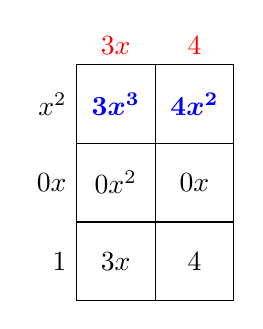
\begin{tikzpicture}
    \draw (0,0) grid (2,3);
    \node at (0,2.5) [left] {$x^2$};
    \node at (0,1.5) [left] {$0x$};
    \node at (0,0.5) [left] {$1$};
    \node at (0.5,2.5) {\color{blue}$\bm{3x^3}$};
    \node at (1.5,2.5) {\color{blue}$\bm{4x^2}$};
    \node at (0.5,1.5) {$0x^2$};
    \node at (1.5,1.5) {$0x$};
    \node at (0.5,0.5) {$3x$};
    \node at (1.5,0.5) {4};
    \node at (0.5,3) [above] {\color{red}$3x$};
    \node at (1.5,3) [above] {\color{red}$4$};
\end{tikzpicture}
\end{center}

Combining like terms inside the boxes, our remainder must be $-2x + 3$. This makes our final answer
\[
\boxed{3x + 4 + \frac{-2x+3}{x^2+1}}
\]

% (d) \quad   $(x^5 + 4x^3 + 2x^2 + 7) \div (x^2 - x + 1)$    \newline\\

% Filling in the missing terms of the dividend, we get the following equivalent problem:
% \[
% (x^5 + 0x^4 + 4x^3 + 2x^2 + 0x + 7) \div (x^2 - x + 1)
% \]

% \begin{center}
%     \begin{tikzpicture}
%     \draw (0,0) grid (4,3);
%     \node at (0,2.5) [left] {$x^2$};
%     \node at (0,1.5) [left] {$-x$};
%     \node at (0,0.5) [left] {$1$};
%     \node at (0.5,2.5) {\color{blue}$\bm{x^5}$};
%     \node at (1.5,2.5) {\color{blue}$\bm{x^4}$};
%     \node at (2.5,2.5) {\color{blue}$\bm{4x^3}$};
%     \node at (3.5,2.5) {\color{blue}$\bm{5x^2}$};
%     \node at (0.5,1.5) {$-x^4$};
%     \node at (1.5,1.5) {$-x^3$};
%     \node at (2.5,1.5) {$-4x^2$};
%     \node at (3.5,1.5) {$-5x$};
%     \node at (0.5,0.5) {$x^3$};
%     \node at (1.5,0.5) {$x^2$};
%     \node at (2.5,0.5) {$4x$};
%     \node at (3.5,0.5) {$5$};
%     \node at (0.5,3) [above] {\color{red}$x^3$};
%     \node at (1.5,3) [above] {\color{red}$x^2$};
%     \node at (2.5,3) [above] {\color{red}$4x$};
%     \node at (3.5,3) [above] {\color{red}$5$};
%     \end{tikzpicture}
% \end{center}

% Combining like terms inside the boxes, our remainder will be $x + 2$. \newline\\

% Thus, the solution is $\boxed{x^3 + x^2 + 4x + 5 + \frac{x+2}{x^2-x+1}}$

% \fi
